%!TEX root = ../thesis.tex
%*******************************************************************************
%****************************** Second Chapter *********************************
%*******************************************************************************

\chapter{The nEDM@SNS Experiment}
\label{ch:nEDM}


\ifpdf
    \graphicspath{{figures/chapter2-figs/}{Chapter2/Figs/PDF/}{Chapter2/Figs/}}
\else
    \graphicspath{{Chapter2/Figs/Vector/}{Chapter2/Figs/}}
\fi

\afterpage{
\begin{figure}
    \centering
    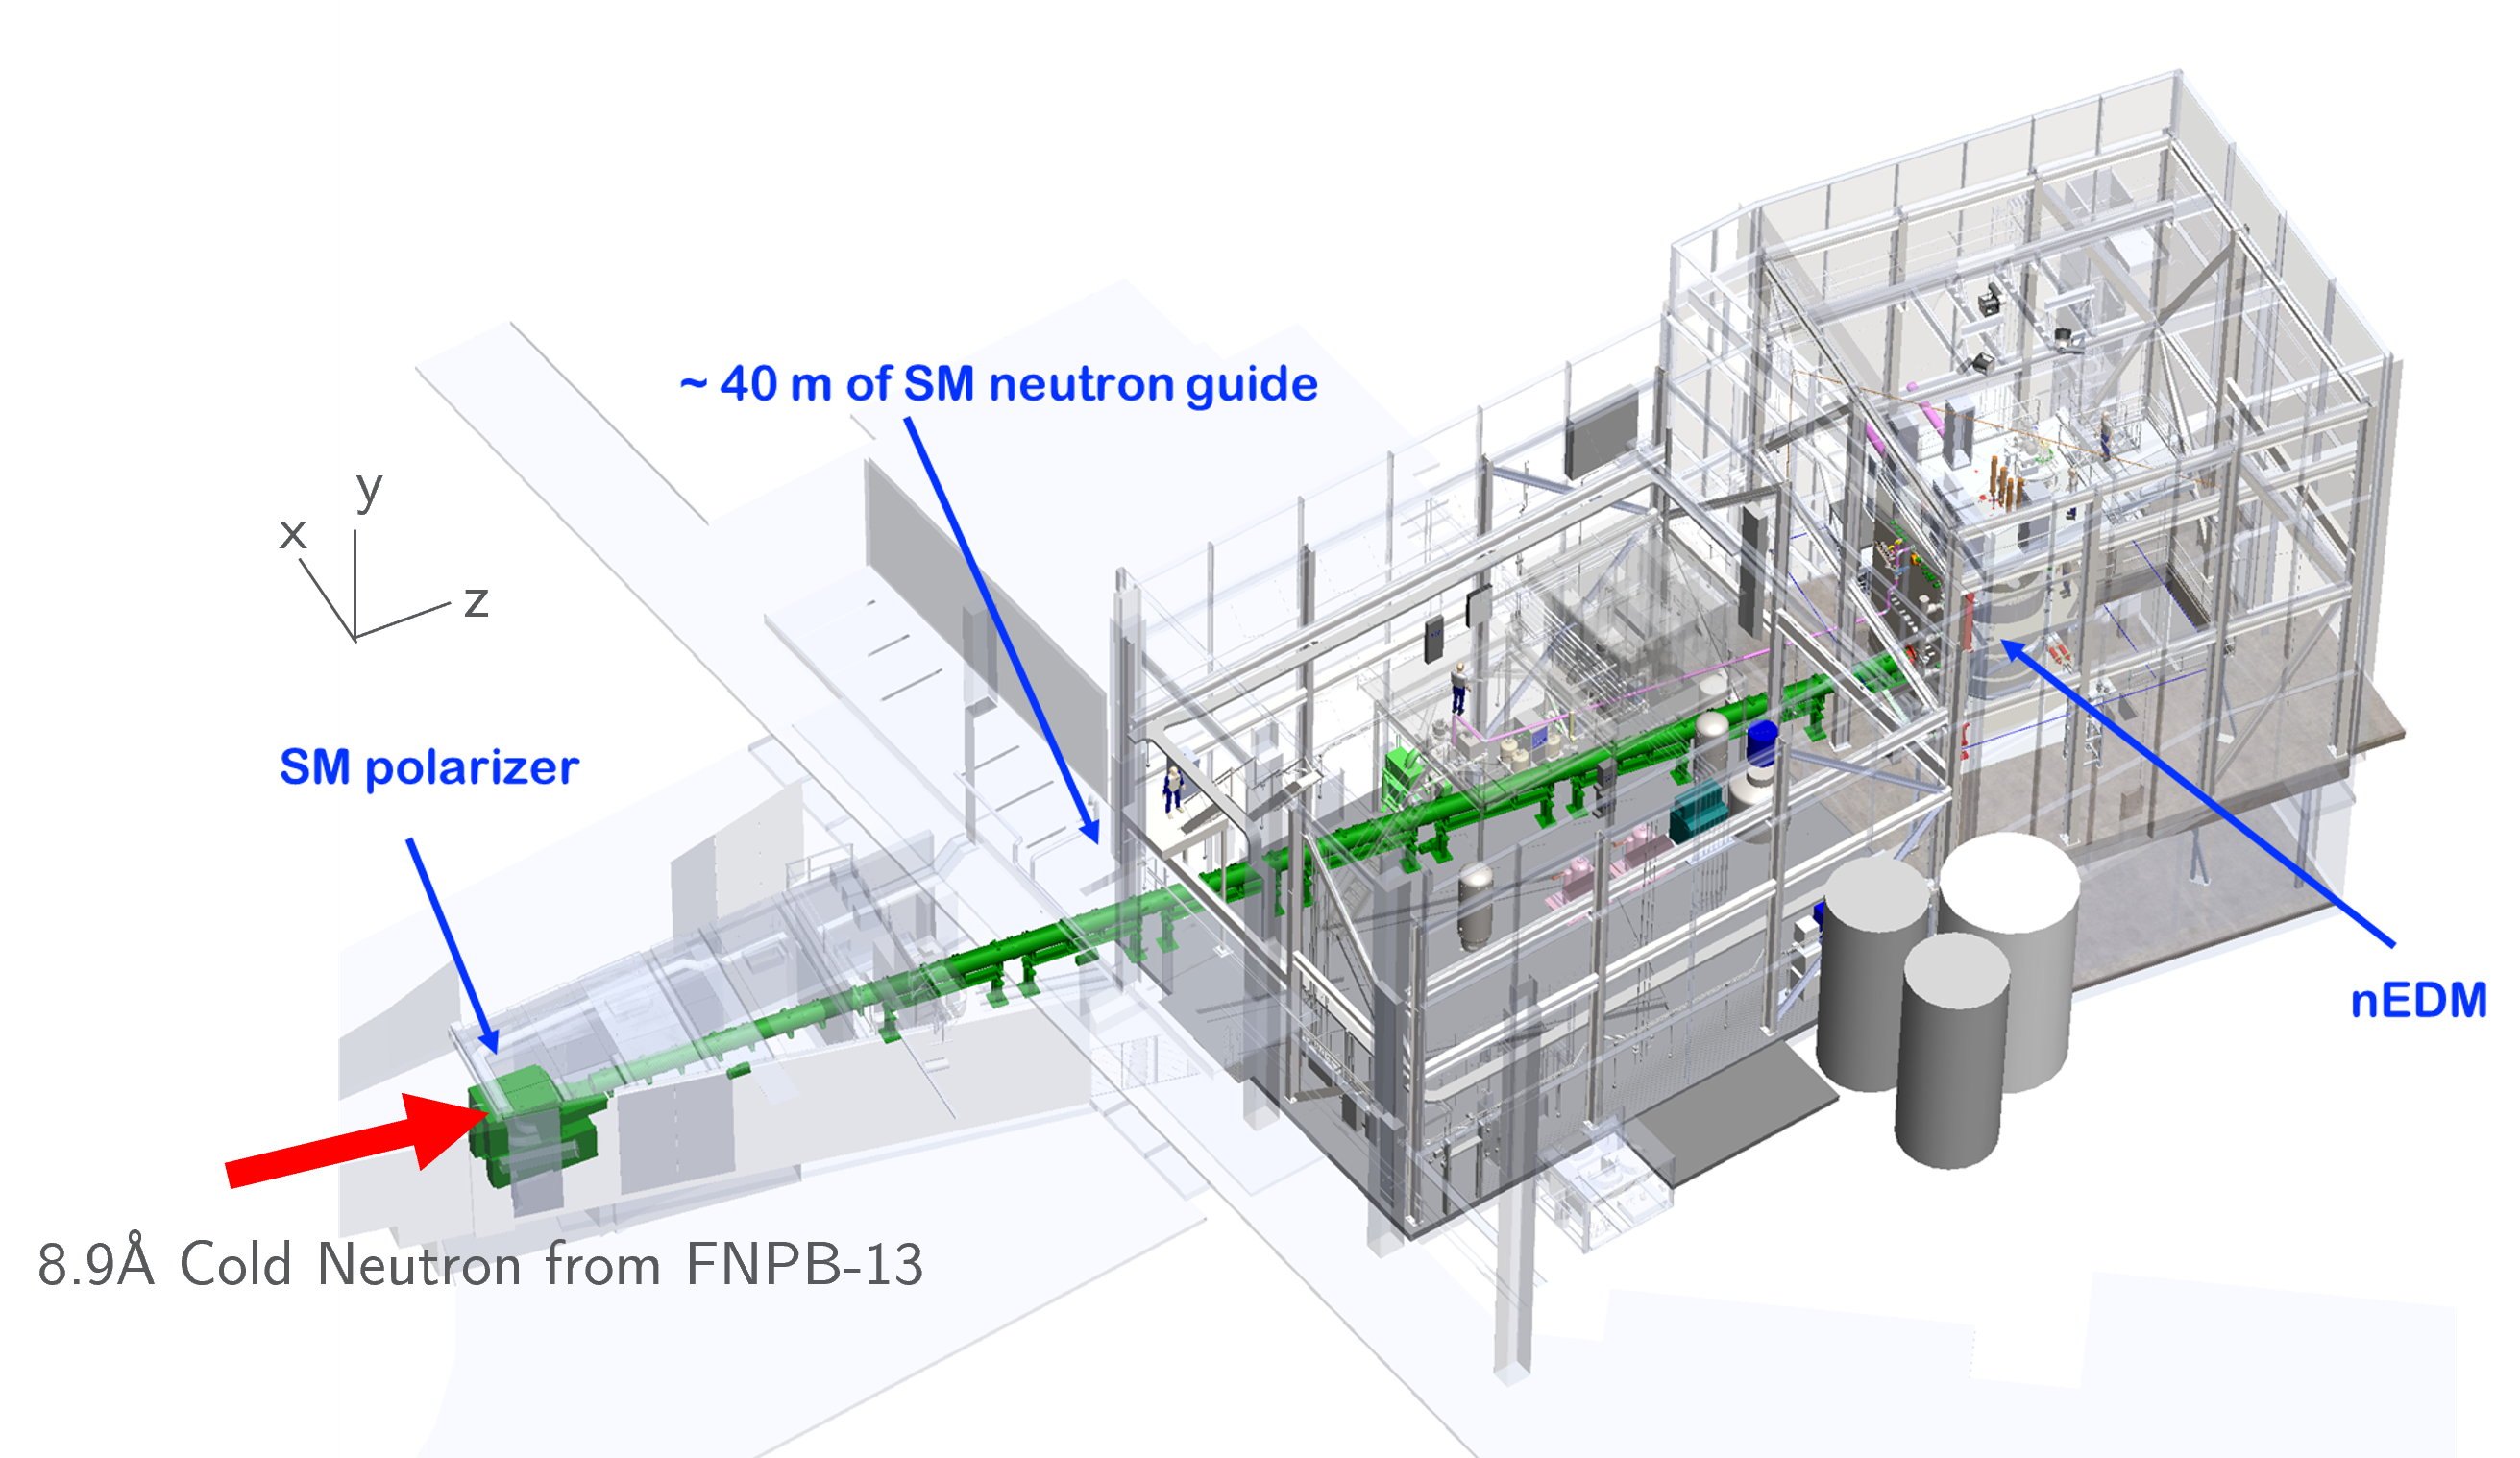
\includegraphics[width=1\textwidth]{figures/chapter2-figs/nEDM_SNS_entire_experiment.png}
    \caption{Schematic overview of the nEDM@SNS experimental apparatus at the Spallation Neutron Source FNPB 13. Figure courtesy of Wolfgang Korsch of the nEDM@SNS collaboration.}
    \label{fig:full_nEDM@SNS}
\end{figure}
\clearpage}

It is clear from the theoretical motivation and the experimental limitations mentioned in \cref{ch:intro} that pioneering experiments are needed to push the sensitivity for the nEDM. In this chapter, the nEDM@SNS experiment, a novel cryogenic apparatus with the goal of improving the nEDM sensitivity, housed at the Spallation Neutron Source (SNS), is described. A schematic overlay nEDM@SNS experiment is shown in \cref{fig:full_nEDM@SNS}. The overall physics of the experiment, the measurement scheme to achieve the expected sensitivity and the major component of the experimental apparatus are described.

\section{Overview}

This experiment, based on the a concept proposed in Ref.~\cite{Golub1994}, makes use of polarized UCN's and polarized $^3$He in superfluid $^4$He. The superfluid $^4$He is used to produce a high density of UCNs in a pair of measurement cells. With this in situ UCN production, the problems of UCN intensity loss that take place for nEDM experiments with external UCN source are avoided. The experiment, uses polarized $^3$He, as a co-magnetometer as well as a live in situ UCN spin analyzer. By contrast, the separated oscillatory fields NMR techniques used in other nEDM experiments analyze the spin precession externally and at the end of the measurement period, leading to statistical sensitivity loss. The superfluid $^4$He is also used as a dielectric insulator allowing for significantly higher electric fields \cite{Ito2016}. These innovative features provide the experiment's ultimate statistical sensitivity for the nEDM as 3-6~$\times$~10$^{-28}$~e~$\cdot$~cm, two order of magnitude better compared to the current nEDM sensitivity.

\afterpage{
\begin{figure}
    \centering
    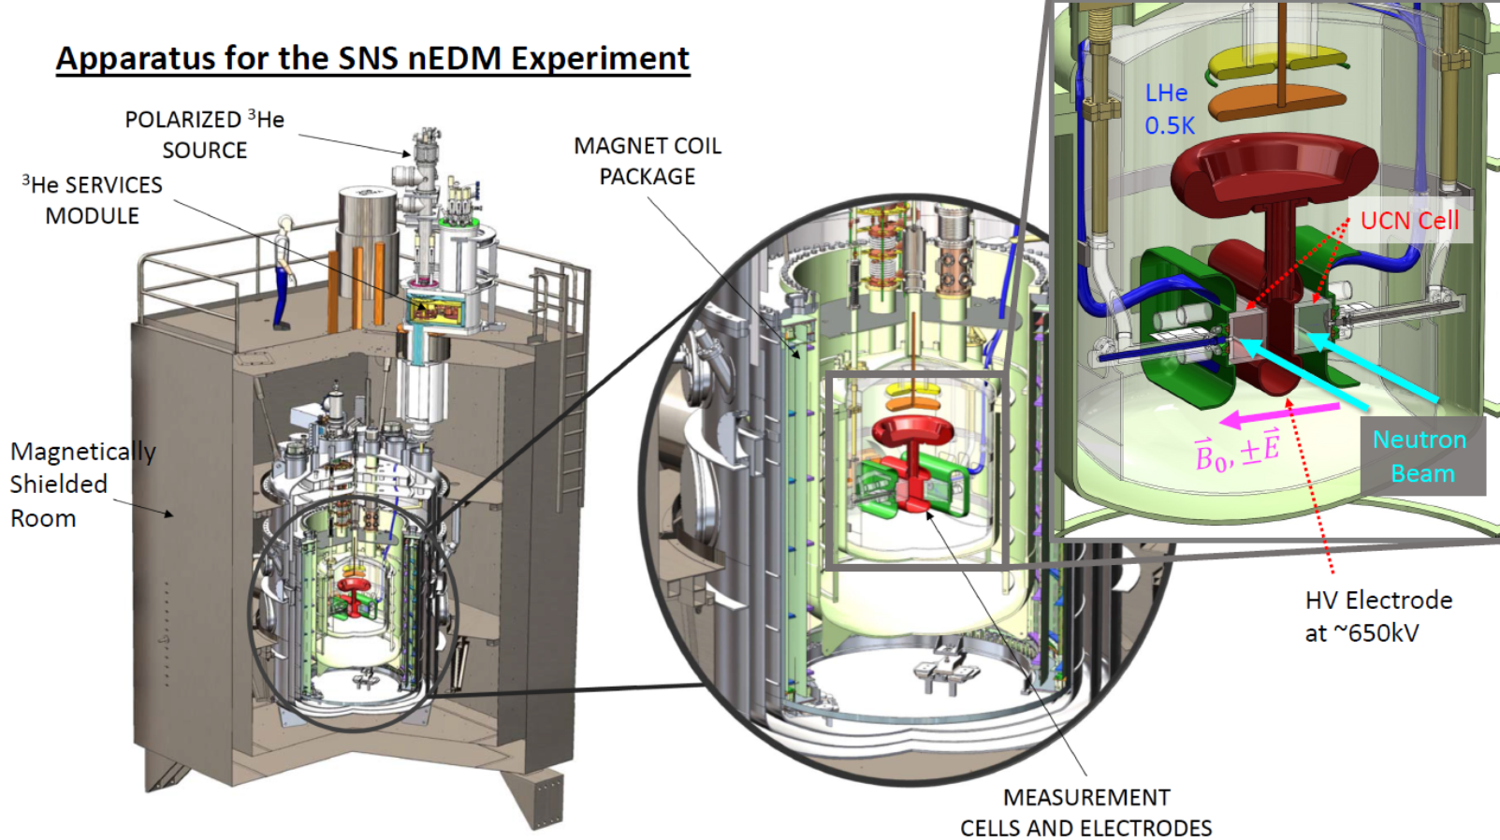
\includegraphics[width=1\textwidth]{figures/chapter2-figs/nEDM_SNS_detail_experiment.png}
    \caption{A detailed schematic overview of the nEDM@SNS experimental apparatus.}
    \label{fig:nEDM@SNS_detail}
\end{figure}
\clearpage}

%The experiment will produce UCN via super-thermal scattering of incoming polarized cold neutrons ($\lambda$ $\sim$ 8.9 \AA) off of phonons in superfluid $^4$He \cite{GOLUB1977337}. UCN's can be confined to a storage volume made of materials with a Fermi potential less than 165 neV. With now experimentally realizable cryogenic temperatures (T $<$ 0.7K) and appropriate materials for storage cells, UCNs can be stored in $^4$He for long periods of time. This, coupled with the fact that superfluid He has large dielectric breakdown strength and hence allows for application of large electric fields \cite{ITO16}, maximizes E$_0$, $\tau$ and $N$ in eq. \ref{eq:uncertainty}. nEDM@SNS will apply B$_0$ = 30 mG and E$_0$ = 75 kV/cm to measure the larmor frequency in eq. \ref{eq:larmor}.

%$^3$He has a spin-dependent neutron absorption cross section, 5300 barns at 1.8\AA \, for anti-parallel neutron and $^3$He spins, increasing as $1/v$, where $v$ is the velocity of neutrons, and nearly zero for parallel neutron and $^3$He spins. For 8.9\AA\ neutrons, the n-$^3$He capture cross section rises to $\sim$26200 barns. For very low concentrations, polarized $^3$He atoms can remain in solution of liquid $^4$He for long periods of time i.e. longer than the neutron's lifetime. The reaction is shown in eq. \ref{abseq}. The energy released from n-$^3$He capture decay products is transferred to the surrounding superfluid $^4$He, which produces ultraviolet (80 nm) scintillation light. Because of the spin dependence of the neutron-$^3$He absorption cross section, the absorption rate of n-$^3$He precessing system is proportional to $1-P_nP_3\cos{\theta_{n3}(t)}$, where $\theta_{n3}(t)$ is the time-dependent angle between UCN and $^3$He polarization, $P_n$ and $P_3$, respectively. The scintillation light will be utilized as the detection mechanism for this variation in n-$^3$He absorption rate. The fact that nEDM@SNS uses in situ spin analysis techniques provide a large increase is statistical sensitivity compared to nEDM experiments that use external spin analysis systems.
%\begin{equation}
%n + {^3He} \rightarrow p+{^3}H+765 \ keV
%\label{abseq}
%\end{equation}
%According to eq. \ref{eq:larmor}, changes in the Larmor frequency, due to the magnetic interaction of $\mu_n$ with magnetic field fluctuations, will decrease the sensitivity of nEDM. Therefore, the nEDM@SNS sensitivity goal necessitates meticulous control of magnetic field fluctuations. Even under such control, magnetic field gradients are expected but can be taken into account using magnetometry. In principle, this magnetometer should provide the average magnetic field over the volume where the neutron precession is taking place. Since the polarized $^3$He has a rapid diffusion time \cite{}, will be exposed to the same magnetic field as UCNs, will be occupying the same volume as the UCN and because the static electric dipole moment of $^3$He is highly suppressed from electron screening \cite{FLAM07}, nEDM@SNS experiment will utilize polarized $^3$He as a co-magnetometer as well. 

%nEDM@SNS will use two frequency measurement techniques. The first method will measure an electric field dependent shift in the scintillation beat frequency. Electric and magnetic fields will be applied to the storage cell parallel to the initial polarization. A $\pi/2$ flip will rotate the spins into a plane perpendicular to the fields. The precession frequency of $^3$He will be measured using SQUID sensors. Since there is a 10\% difference in the gyromagnetic ratios of UCN ($\gamma_n$), and $^3$He ($\gamma_3$), the variation in scintillation rate will be the beat frequency $\Delta\omega = B_0 (\gamma_n - \gamma_3)$. 
%\begin{equation}
 %   \omega_{n3} = \left(\gamma_n - \gamma_3\right) \frac{\omega_3}{\gamma_3} %\pm \frac{2d_nE_0}{\hbar}
%\end{equation}
%The neutron precession frequency shift can then be extracted if the $^3$He precession frequency is added to the scintillation beat frequency, $\omega_{n3}$.  Thus, using the neutron precession frequency under different directions of the electric field, the nEDM can be extracted. Thus, the polarized $^3$He will act as a live in situ co-magnetometer and spin polarization analyzer,

%The second method, called critical spin dressing, involves applying an AC magnetic field, forcing the UCN and $^3$He to precess at the same effective precession frequency.
%\begin{equation}
 %   \omega_n-\omega_3 = \gamma_nJ_0(x_n)-\gamma_3J_0\left(\frac{\gamma_3}{\gamma_n}x_n\right) = 0
%\end{equation}
%where $J_0$ is the zeroth order Bessel function of first kind and $x_n = \gamma_n \frac{B}{\omega}$, where $B$ and $\omega$ are the magnitude and frequency of applied AC magnetic field. $B$ and $\omega$ can be selectively tuned at critical dressing parameter, $x_n$, such that in the absence of an electric field, $\Dot{\theta}_{n3}(t) = 0 $ therefore the scintillation rate will be constant. In the presence of an electric field and a non-zero nEDM, $\theta_{n3}$ will be modified as 
%\begin{equation}
 %   \theta_{n3}(t) = \pm\phi_0 \pm \frac{2J_0(x)d_{n}E}{\hbar}t
%\end{equation}
%where $\phi_0$ is the initial angle between spins, therefore scintillation rate will no longer be constant. This method eliminates the need for $^3$He co-magnetometry.  By utilizing both methods, possible unknown systematic effects can be uncovered.

%The nEDM@SNS experiment will employ a multi-pronged strategy to shield against external fields: external field cancellation coils, room-temperature shielding and superconducting shielding \cite{Ahmed_2019}. As shown in figure \ref{fig:2}, the nEDM magnet cryostat magnet, which surrounds the measurement cells, is made of several concentric layers. The components within the cryogenic magnet package work together to provide shielding and generate magnetic fields that satisfy strict uniformity requirements. Since the nEDM@SNS requires the use of polarized neutrons, therefore, both polarization and transport efficiency of the neutron beam through the cryostat and magnet package windows should be maximized to optimize sensitivity.

%\begin{figure}[p]
 %   \centering
 %   \includegraphics[width=.9\textwidth]{cryogenicapparatus.png}
  %  \caption{A schematic overview of the nEDM@SNS cryostat magnet package. The enlarged section shows the beam windows the incoming polarized neutrons will pass through.}
   % \label{fig:2}
%\end{figure}

\Cref{fig:nEDM@SNS_detail} shows a detailed view of the nEDM@SNS experiment. The Larmor precession measurement, as shown in \cref{eq:larmor}, for the nEDM@SNS experiment will take place inside two measurement cells at the center of the apparatus made of deuterated polystyrene (dPS) plus deuterated tetraphenyl butadiene (dTPB) and acrylic. These cells will be filled with isotopically purified superfluid $^4$He 0.4 K. A highly homogeneous magnetic field, $B_0$, of magnitude 30 mG will be applied along the transverse direction of the measurement cells (parallel to horizontal axis). This field is selected to provide control over the systematic effects arising from magnetic field gradients. Highly Polarized $^3$He ($P_3 \sim 0.98$) , polarized parallel to $B_0$ field, at an isotropic concentration of $x_3 \sim 10^{-10}$ (atomic density of $10^{12}$ cm$^{-3}$), as compared to the natural abundance of $^3$He ($x_3 \sim 10^{-3}$ to $10^{-6}$), will be loaded into the measurement cells. A high voltage electrode, situated in between the two measurement cells and two ground electrodes flanking the measurement cells will be used to provide an electric field parallel to $B_0$ for one cell and antiparallel to $B_0$ in the other cell. The electrodes will provide an expected electric field magnitide of $E_0$ = 75 kV cm$^{-1}$. This high electric field is achievable due to the high dielectric breakdown strength of superfluid helium. 

The measurement cells will be illuminated with polarized 8.9~\AA\ neutrons, which undergo down-scattering in superfluid $^4$He via phonon emission in a process called superthermal scattering, to produce UCNs \cite{Golub1977, Golub1983, Golub1975}. The FNPB neutron beamline 13 with time of flight choppers will be used to provide the monochromatic 8.9~\AA\ neutrons with $\Delta \lambda / \lambda $ of 0.01 to suppress non-UCN converted neutron backgrounds. The monochromatic neutrons will be polarized parallel to the $B_0$ field direction, via a supermirror neutron polarizer ($P_n$ = 0.98) and transported to the measurement cells via neutron guides with spin transport magnetic fields. The UCN polarization is expected to be at the same level since the superthermal process does not cause a change in angular momentum and the spin dependent capture interaction of neutrons and $^3$He eliminates any undesired UCN polarization. The inner walls of the measurement cells will be coated with deuterated polystyrene with a neutron optical potential of $\sim160$ neV. The UCN production rate based on the measurement cell design is expected to be $\approx$ 0.31 UCN cm$^{-3}$ s$^{-1}$.

The UCN density build up, time $\tau_{UCN}$, over the course of the monochromatic neutron beam illumination will be dictated by:
\begin{equation}
    \frac{1}{\tau_{UCN}} = \frac{1}{\tau_{\beta}} + \frac{1}{\tau_{up}} + \frac{1}{\tau_{wall}} + \frac{1}{\tau_{n3}}
    \label{eq:UCN_losstime}
\end{equation}
where:
\begin{itemize}
    \item $\tau_{\beta}$ is the mean neutron $\beta$-decay lifetime of 878 s \cite{PDG2022}. 
    \item $\tau_{up} $ is the UCN loss time from upscattering with the superfluid $^4$He and is expected to be about $ 6 \times 10^4$ s at 0.4 K \cite{Golub1983, Golub1979, Ye2009}.
    \item $\tau_{wall}$ is the UCN loss time from measurement cell wall collisions, and is expected to be $ > $ 2000 s based on the measurement cell design.
    \item $\tau_{n3}$ is the UCN-$^3$He absorption time, which can be chosen to optimize sensitivity.
\end{itemize}
Based on this UCN built up time, the maximum achievable UCN density in each cell is expected to be $\approx$ 170 UCN cm$^{-3}$ or about $5\times10^5$ UCNs per measurement cell. Even at $x_3 \sim 10^{-10}$ concentrations levels, polarized $^3$He can remain in the solution of liquid $^4$He for much longer than the UCN lifetime.

\section{Measurement Technique}

$^3$He has a spin-dependent neutron absorption reaction with a strong preference for anti-parallel neutron and $^3$He spin capture \cite{Passell1966}. The spin averaged cross section is 5300 barns at 1.8~\AA, increasing as $1/v$, where $v$ is the velocity of neutrons \cite{Mughabghab1981}. The reaction is shown in \cref{abseq}. For UCNs, the n-$^3$He capture cross section rises to $\sim 8\times 10^5$ barns. The energy released from n-$^3$He reaction decay products excites superfluid $^4$He, which upon relaxation, produces ultraviolet (80 nm) scintillation light. This scintillation light is captured by the dTPB in the cell walls and wavelength shifted to blue light, which is then extracted out from the measurements cells via fiber guides as green light. 
\begin{equation}
n + {^3He} \rightarrow p+{^3}H+765 \ keV
\label{abseq}
\end{equation}
The polarized UCNs and polarized $^3$He will precess about the same electric and magnetic fields inside the measurement cells. The scintillation light from the spin dependent capture, which will be proportional $1-P_nP_3\cos{\omega_{n3}(t)}$, will be used to determine the relative beat precession frequency, $\omega_{n3}$, of the two species throughout the measurement run. Since the capture reaction and the spin precession takes place inside the measurement cells, live and in situ the spin analysis will be performed. The time evolving capture rate, $R(t)$, from the scintillation light can be thought of as: 
\begin{equation}
    R(t) = N_0 \frac{\epsilon_{n3}}{\tau_{n3}} \left ( 1-P_n P_3 \cos{(\omega_{n3}t}) \right )
    \label{eq:cap_rate}
\end{equation}
where $N_0$ is the initial number of UCNs and $\epsilon_{n3}$ is the capture scintillation detection efficiency.
The live in situ spin analysis will be performed using two measurement schemes: free precession and spin critical dressing. In both schemes, The measurement cycle begins after the measurement cells are filled with UCNs. An RF magnetic field is used to apply a $\pi$/2 pulse on the polarized UCN and $^3$He for spin precession in the plane transverse to $B_0$ and $E_0$.


\subsection{Free Precession}

In the free precession mode, the UCNs and $^3$He in both cells are left to precess uninterrupted. Based on the Larmor precession of UCN and $^3$He under the application of $B_0$ and parallel(+)/antiparallel(-) $E_0$, the relative beat frequency $\omega_{n3}$ between UCN and $^3$He forms as: 
\begin{equation}
    \omega_{n3}t + \phi_0 = \left( \left(\gamma_n - \gamma_3 \right) B_0 \pm \frac{2d_nE_0}{\hbar} \right) t + \phi_0
    \label{eq:fp_pres}
\end{equation}
where $\gamma_n = -1.8 \times 10^4$ rad s$^{-1}$ G$^{-1}$ \cite{Codata2021} and $\gamma_3 = -2.0 \times 10^4$ rad s$^{-1}$ G$^{-1}$ \cite{Codata2021} are the neutron and $^3$He gyromagnetic ratios, respectively, and $\phi_0$ is the initial phase of the UCN and $^3$He precession. For $B_0$ = 30 mG, $\omega_{n3}/2\pi$ = -9.8 Hz \footnote{A negative sign comes from the fact that $\gamma_n$ and $\gamma_3$ are negative and precess in counterclockwise direction when looking parallel to the $B_0$ axis.}. 


From the expected spin relaxation of the precessing UCNs and $^3$He over time as well as the UCN loss time in \cref{eq:UCN_losstime}, the scintillation light event rate from the free precession mode will be: 
\begin{equation}
 R(t) = N_0 e^{-t/\tau_{UCN}} \left (\frac{\epsilon_\beta}{\tau_\beta}+\frac{\epsilon_3}{\bar{\tau}_3}\right ) \left [1- \frac{\epsilon_3
P_3P_n}{\bar{\tau}_3\left (\frac{\epsilon_\beta}{\tau_\beta}+\frac{\epsilon_3}{\bar{\tau}_3}\right )} \cos{(\omega_{n3} t+\phi_0 )}
\right ]+ R_{BKGD}
\label{eq:FP_rate}
\end{equation}
The natural beta-decay of UCNs is the largest background source followed by cosmic muons, ambient gamma rays and the scattered neutrons from any wall collisions. The spectrum of the number of scintillation light photons from UCN-$^3$He capture is monoenergetic \cite{Ito2012, Ito2013}, therefore, with selective cuts, non UCN-$^3$He photons can be excluded and any non UCN-$^3$He capture related background events included is $R_{BKGD}$ in \cref{eq:cap_rate}. Based on the design of the scintillation light collection system, the expected efficiency for UCN-$^3$He capture events is $\epsilon_{n3}$ = 0.93 and $\epsilon_{\beta}$ = 0.33 for beta decay events. This decaying scintillation light oscillation signal simultaneously extracted from both measurement cells with parallel/anti-parallel $E_0$ will be numerically fitted to extract the beat frequency $\omega_{n3}$ of both cells.

So far it is assumed that the static $B_0$ field experienced by the two measurement cells is identical. However, since the beat frequency is being extracted over time from spatially apart cells, comagnetometry is required to account for drifts in the magnetic field. Since the precession of the polarized $^3$He in the measurement cells will be affected by magnetic field drifts and gradients, therefore, $^3$He will be used as a comagnetometer. Furthermore, $^3$He has a short diffusion time \cite{Lamoreaux2002}, a small EDM compared to nEDM due to to atomic screening \cite{Dzuba2007, Flambaum2012} and in much larger densities than UCNs, therefore, $^3$He precession will be used to provide a nearly exact spatial\footnote{Technically, there is an offset in the center of gravity between the UCNs and $^3$He, due to a difference in their thermal energies. This means that under the presence of magnetic field gradients, UCNs and $^3$He will have different precession frequencies. This shift can be accounted for using the motional magnetic fields shifts from  reversing the electric field.} and temporal average of the magnetic field affecting the UCNs over the measurement period. The $^3$He precession, $\omega_{3} = \gamma_3 B_0$, will be measured by an array of Superconducting Quantum Interference Device (SQUID) magnetometers adjacent to the measurement cells \cite{Kim2015} simultaneously with the UCN-$^3$He scintillation light. By accounting for the $^3$He precession from the magnetometry in the beat frequency, $ \omega_{n} = \omega_{n3} - \omega_{3} $, the neutron Larmor precession frequency from the parallel and anti-parallel $E_0$ from the two measurement cells will be used to extract the nEDM, $d_n$, as:
\begin{equation}
 \Delta \omega_{n} = \omega_{n}^{+E} - \omega_{n}^{-E} = \frac{4d_nE_0}{\hbar}
\end{equation}


%Monte-Carlo simulations of the scintillation event rate versus time during the free precession period have been made and fitted (see Fig. 2). The fit is performed over the whole free precession measurement time Tm. However, since we are able to observe the live UCN precession with our technique, the frequency analysis can be performed in short time windows. This will be useful for correcting temporal magnetic field drifts (see Sec. 2.3).

%At the end of every measurement cycle, the (partially) depolarized $^3$He will be removed from the cell and new polarized $^3$He injected into the cell (described in Sec. 3). The E field may also be reversed systematically between measurement cycles. The combined time for these operations is the dead time. For the sensitivity discussions next, a dead time of 337 s is assumed, along with an ambient background rate of RBG = 5 s−1 . The influence of these parameters on the sensitivity have been studied. Additionally, φ0 is assumed to be fixed in the fitting routine for the discussions below. This requires φ0 to be reproducible after the π/2 pulse.

Prior to each measurement cycle, the polarized $^3$He will be loaded into the measurement cells. Then, the measurement cells will be loaded with polarized UCNs via the superthermal process. After that, the precession measurement of UCNs and $^3$He will commence until all UCNs are captured. After each measurement cycle time, the depolarized $^3$He is removed, UCNs and polarized $^3$He are reloaded into the measurement cells and the precession measurement is repeated. 

Based on simulations of the optimal experimental parameters, the 1-$\sigma$ level statistical precision on the nEDM from the free precession mode comes out to be around $6 \times 10^{-28}$ e$\cdot$cm i.e. an uncertainty of $\sigma_{\frac{\omega_{n3}}{2\pi}}$ = 1.7 $\mu$Hz. This statistical significance corresponds to around 300 live days of scintillation and SQUID runs with the entire free precession measurement, including operational setup, taking 3 calendar years \footnote{It is worth mentioning that this experiment will achieve a precision of $10^{-27}$ e$\cdot$cm, the precision goal of other nEDM experiments throughout the world, with only a month's worth of data taking.}. 

\subsection{Critically Dressed Spin}

In spin critical dressing technique, after the $\pi$/2 pulse, an RF magnetic field transverse to $B_0$ magnetic field with magnitude, $B_{RF}$, much stronger than $B_0$ and angular frequency, $\omega_{RF}$, off the resonance frequency, $\omega_{L} = \gamma_{n,3} B_0 $, will be applied \cite{Haroche1970, Cohen-Tannoudji1969}. In the limit $\omega_{L} \ll \omega_{RF}$, the RF field will cause the gyromagnetic ratios of both UCNs and $^3$He, $\gamma_{i}$ to be modified to:
\begin{equation}
    \gamma_{n,3}^{eff} = \gamma_{n,3}J_0\left( \gamma_{n,3}\frac{B_{RF}}{\omega_{RF}}\right)
\end{equation}
where $J_0$ is the zeroth-order Bessel function of the first kind. This is called a dressed spin system.

By tuning the dressing RF field, the effective gyromagnetic ratios of the $^3$He and UCNs will be made equivalent, i.e. $\gamma_{n}^{eff} = \gamma_{3}^{eff}$ . For example, this happens for $\gamma_{n}\frac{B_{RF}}{\omega_{RF}} \approx 1.19$,  where $B_{RF}$ = 1 G, a dressing frequency $\omega_{RF}/2 \pi \approx 2.5$ kHz. This is called a critically dressed spin system, where now both polarized UCNs and polarized $^3$He will be precessing at the same relative rate, $\omega_{n3}$. Here, the critically dressed UCN-$^3$He system will become sensitive to magnetic field changes rather than the individual UCN and$^3$He species. The scintillation rate will be constant and dictated by the initial phase, $\phi_0$. In the presence of a non-zero $d_n$, the scintillation rate will then vary under the application of parallel and antiparallel $E_0$, albeit slightly, as:
\begin{equation}
    \omega_{n3}t + \phi_0 = \left(  \pm \frac{2d_nJ_0E_0}{\hbar} \right) t + \phi_0
\end{equation}

As of yet, the scintillation rate signal will be a featureless decaying distribution, making it difficult to compare the fits on the scintillation signal from the different measurement runs. In order to compare measurement runs, the scintillation rate will be converted into an time-dependent asymmetry measurement based on the phase accumulated due to a non-zero nEDM. To do this, a modulation scheme will be applied to change the initial angular phase, $\phi_0$, periodically between  $- \phi_0$ and $\phi_0$, the scintillation rate will then vary as:
\begin{equation}
    \omega_{n3}t \pm \phi_0 = \left(  \pm \frac{2d_nJ_0E_0}{\hbar} \right) t \pm \phi_0
\end{equation}
By measuring the scintillation rate for the two phases of the measurement cycle as $R_+$ and $R_-$ for for equal amounts of time, $\Delta t$, a time dependent rate asymmetry, $A_{d_{n}}(\Delta t)$, will be used to extract the nEDM, $d_n$, as:
\begin{equation}
    A_{d_{n}}(\Delta t)= \frac{R_+-R_-}{R_++R_-}
\end{equation}
where
\begin{equation}
    R_{\pm}(\Delta t) = N_0 e^{-\frac{\Delta t}{\tau_{UCN}} } \left [ \frac{ \epsilon_\beta}{\tau_\beta} + \frac{\epsilon_3}{\bar{\tau}_3} \left(1-P_3P_n\cos \left(  \pm \frac{2d_nJ_0E_0}{\hbar}  t \pm \phi_0 \right) \right) \right] + R_{BKGD}
\end{equation}
and
\begin{equation}
 \frac{1}{\tau_{UCN}} =\frac{1-P_3P_n\cos\left(  \pm \frac{2d_nJ_0E_0}{\hbar}  t \pm \phi_0 \right)}{\tau_{n3}}
+\frac{1}{\tau_\beta}+\frac{1}{\tau_{cell}}+\frac{1}{\tau_{up}}
\end{equation}

Assuming optimal parameters, 1-$\sigma$ statistical precision from the critical dressed spin mode with modulation is expected to be $3 \times 10^{-28}$ e$\cdot$cm \cite{Ahmed2019}. This statistical significance corresponds to around 300 live days of scintillation runs with the entire measurement, including operational setup, taking 3 calendar years. Primary reason for improvement of statistical sensitivity is because the UCNs last longer, as their spins are never anti-parallel, since the technique allows for a control of the relative precession of UCN-$^3$He system. Since critical dressing makes the combined UCN-$^3$He system sensitive to magnetic field changes rather than the individual species, this eliminates some of the systematic effects associated with $^3$He SQUID comagnetometry in free precession mode. Conveniently, having two independent measurement techniques allows for a check on the different systematic effects from the two measurement modes. Due to the intricacies of the critically dressed spin technique, the Systematics and Operation Studies apparatus \cite{Ahmed2019} will be used to study the UCN and $^3$He critical dressing as well as various modulation techniques, as described in \cite{Swank2018, Ahmed2019, Tat2022}, to understand the effects on the statistical sensitivity and any suppression of systematic effects.

\subsection{Systematical Effects}

Despite the meticulous control and characterization techniques of the magnetic fields employed in this experiment, systematic uncertainties on the nEDM measurement are bound to exist and must be suppressed in order to further search for new physics.

The largest systematic effect arises from the geometric phase of the precession in the effective magnetic field created by the $B_0$ magnetic field gradients and the motional magnetic field, $B_{E \times v} = E \times v/c^2$ , leading to frequency shifts proportional the electric field, $E$, i.e. false nEDM signal, called the Bloch-Siegert false EDM \cite{Bloch1940, Pendlebury2004}. The size of this frequency shift depends on the size of the field gradients, the collisional motion of the particle, and the dimensions of the measurement cell. Both the neutron and $^3$He will exhibit this frequency shift, although the shift is much larger for $^3$He because of the differences in the motion ($^3$He atoms undergo diffusive motion in superfluid $^4$He with the mean free path scaling with temperature as $ \sim T^{-7.5}$ \cite{Baym2013}) and the precession since $ \frac{\gamma_3}{\gamma_n} \approx 1.1$.

One method to characterize and suppress this false EDM effect is to perform a scan by intentionally introducing magnetic field gradients and interpolating until the total gradients are negligible \cite{Pendlebury2015}. Since the $^3$He undergoes a strong temperature dependent diffusive motion, the temperature of the superfluid helium will be tuned as well to control this effect for the comagnetometer and characterize any magnetic field gradients. This gradient-temperature technique will be further explored at the Systematics and Operation Studies apparatus as well \cite{Ahmed2019, Swank2012, Swank2016}. 

\section{Apparatus}

A schematic overview of the key nEDM@SNS experimental apparatus is shown in \cref{fig:key_nEDM@SNS}. The main subsystems that make up the apparatus are: the Central Detector System, the $^3$He Services System and the Magnetic Field Module System including the Magnetic Shielding Enclosure. Presently, these subsystems are being researched and developed at the different collaborating institutions before their eventual assembly and commissioning at the SNS as shown in \cref{fig:key_nEDM@SNS} and \cref{fig:full_nEDM@SNS}. This section gives a brief overview of each of subsystem. A more detailed overview can be found in \cite{Ahmed2019}.

\afterpage{
\begin{figure}
    \centering
    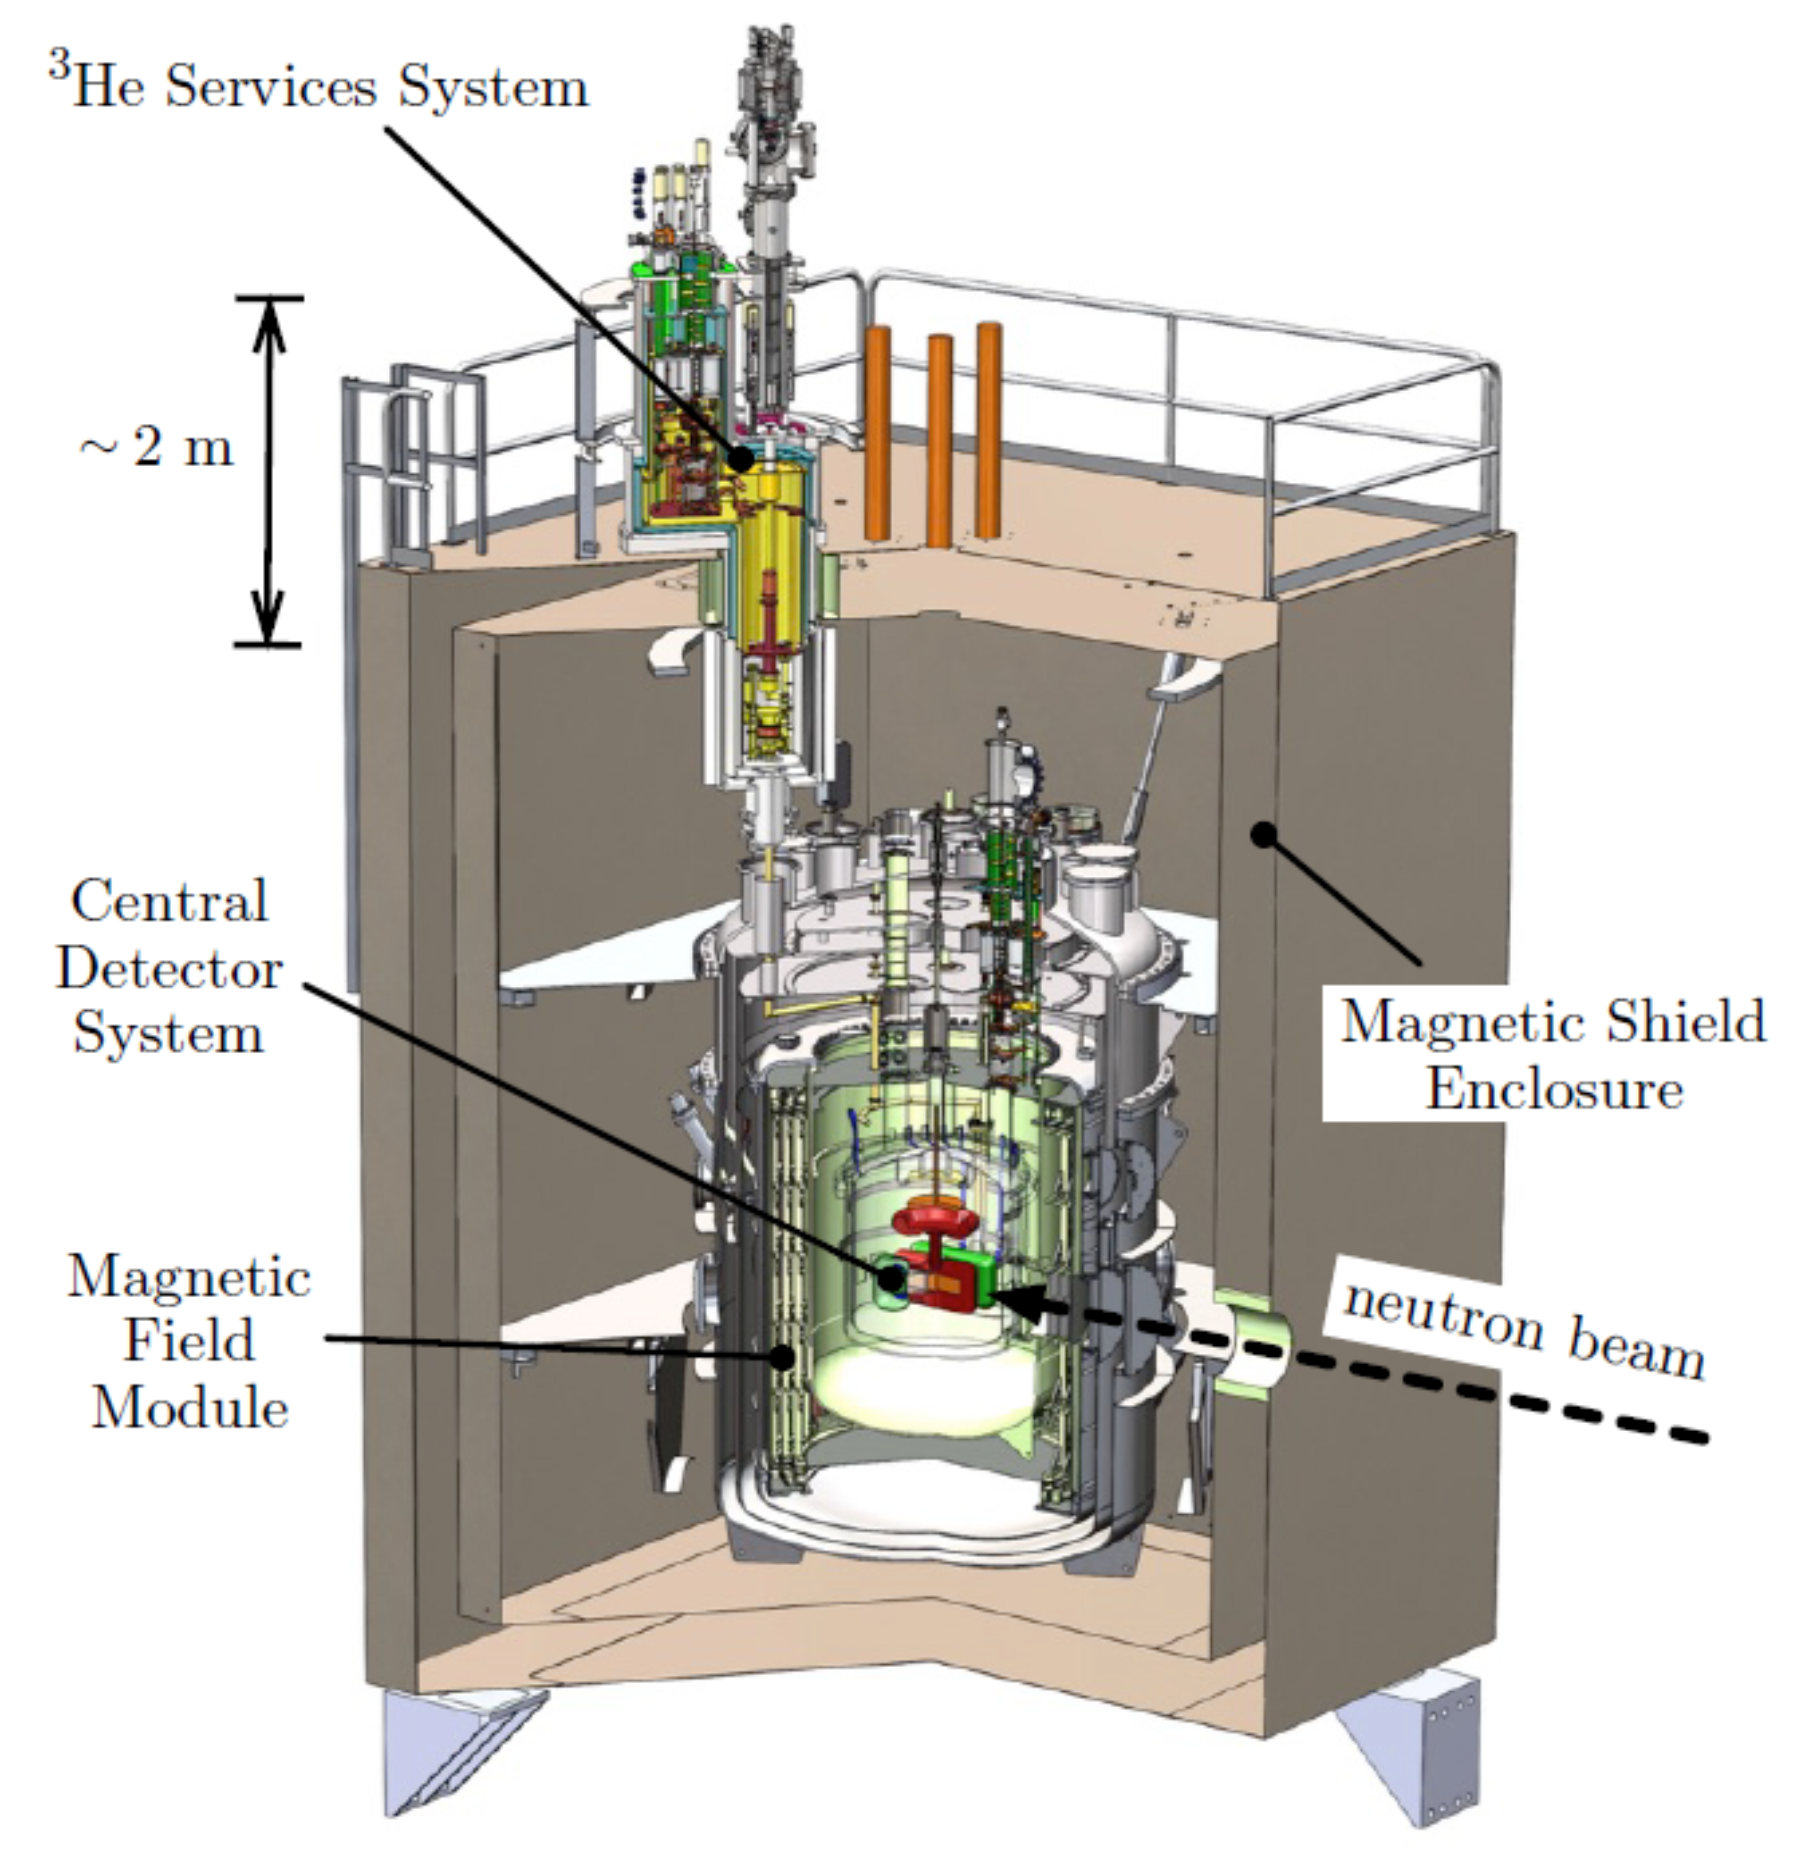
\includegraphics[width=1\textwidth]{nEDM_SNS_experiment.png}
    \caption[Schematic overview of the key nEDM@SNS experimental apparatus.]{Schematic overview of the key nEDM@SNS experimental apparatus. Figure taken from \cite{Ahmed2019}.}
    \label{fig:key_nEDM@SNS}
\end{figure}
\clearpage}

\subsection{Central Detector system}

The Central Detector System (CDS), shown in greater detail in \cref{fig:CDS}. The CDS volume is made of fiberglass composite which will be filled 1600 L of superfluid helium and cooled to 0.4~K with a non-magnetic dilution refrigerator (DR). The purpose of the CDS is to harbor the two measurement cells, the high voltage electrode system, SQUID magnetometers array, and the  scintillation light collection fibers. The entire CDS volume along with its inner components is made of non-magnetic materials to prevent field gradients and non-electrically conductive materials to prevent the thermal ringing noise in the SQUIDS as well as eddy current heating from the RF magnetic fields. 

\afterpage{
\begin{figure}
    \centering
    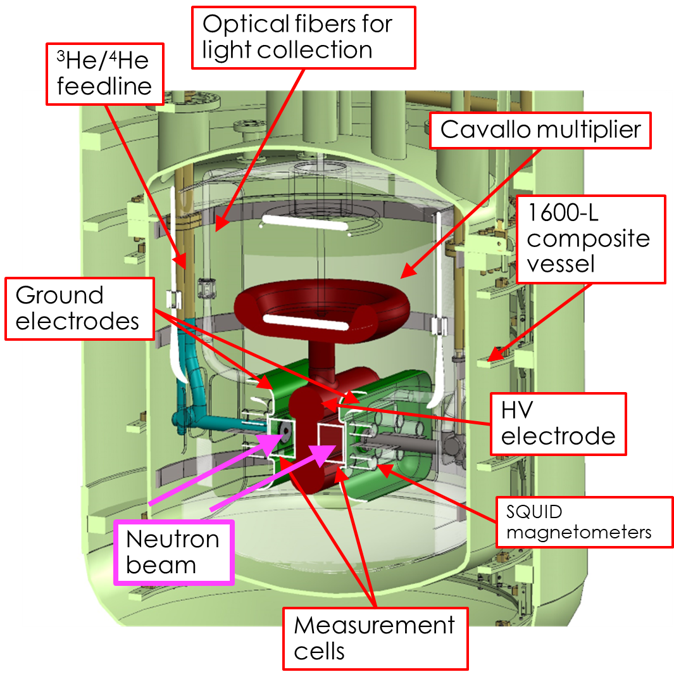
\includegraphics[width=1\textwidth]{figures/chapter2-figs/CDS_detail.png}
    \caption{A detailed view of the Central Detector System (CDS). Figure courtesy of Takeyasu Ito of the nEDM@SNS collaboration.}
    \label{fig:CDS}
\end{figure}
\clearpage}

As stated earlier, the measurement cells will be composed of acrylic PMMA with inner walls coated in highly pure deuterated polystyrene (dPS) with embedded deuterated tetraphenyl butadiene (dTPB). The cell will be 40 cm long, 7.5 cm wide and 10 cm tall with a wall thickness of 1.2 cm. The cell materials are deuterated to allow for UCN production as well as provide a long UCN storage time by preventing upscattering of UCNs. The purpose of dTPB is to wavelength shift the scintillation light for collection and extraction by the light fibers guides \cite{McKinsey1997}. A deuterated plastic valve in between the two cells will allow (un)loading of (de)polarized $^3$He into the measurement cells. 

The high voltage electrodes will be made of PMMA with electrically conductive coating. The desired 75 kV/cm electric field corresponds to a potential of 630 kV of the longitudinal area of the cell. A cryogenic high voltage amplification system, called the Cavallo multiplier, will be used to provide the large electric potential \cite{Ahmed2019}. The operating principle of electrostatic charge transfer based on the relative capacitance of each of the electrodes in the amplification process is shown in \cref{fig:Cavallo}.

\afterpage{
\begin{figure}
    \centering
    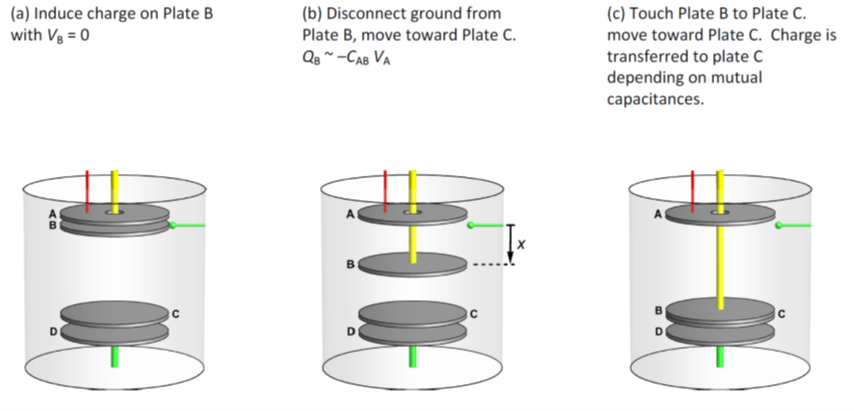
\includegraphics[width=1\textwidth]{figures/chapter2-figs/Cavallo_schematic.png}
    \caption[A schematic showing the operating principle of Cavallo high voltage amplification system design for the nEDM@SNS experiement.]{A schematic showing the operating principle of Cavallo high voltage amplification system design for the nEDM@SNS experiement. Figure taken from \cite{Ahmed2019}.}
    \label{fig:Cavallo}
\end{figure}
\clearpage}

\subsection{Polarized ${^3}$He System}

The polarized $^3$He system, as shown in \cref{fig:3He_sys}, will be located atop the CDS as shown in \cref{fig:key_nEDM@SNS}. The polarized $^3$He system has three functions for the operation of the nEDM@SNS experiment: (i) polarize the $^3$He, (ii) inject the polarized $^3$He into the measurement cells and (iii) remove the depolarized $^3$He from the measurement cells \cite{Ahmed2019}.

$^3$He will be polarized using an atomic beam source (ABS) \cite{Esler2007, Eckel2012}. This cryocooled $^3$He source uses inhomogeneous magnetic fields from a quadrupole magnet to filter out one spin state, polarizing the $^3$He atoms \cite{Ahmed2019}. The polarized $^3$He will be injected into the measurement cell by applying temperature gradients which induce phonons (‘heat flush’) that will carry the polarized $^3$He \cite{Baym2015}. This polarization will be adiabatically maintained via spin transport magnetic fields. After the spin precession measurement is finished, the depolarized $^3$He will be removed via the heat flush technique into a separate volume, to be discarded. 

\afterpage{
\begin{figure}
    \centering
    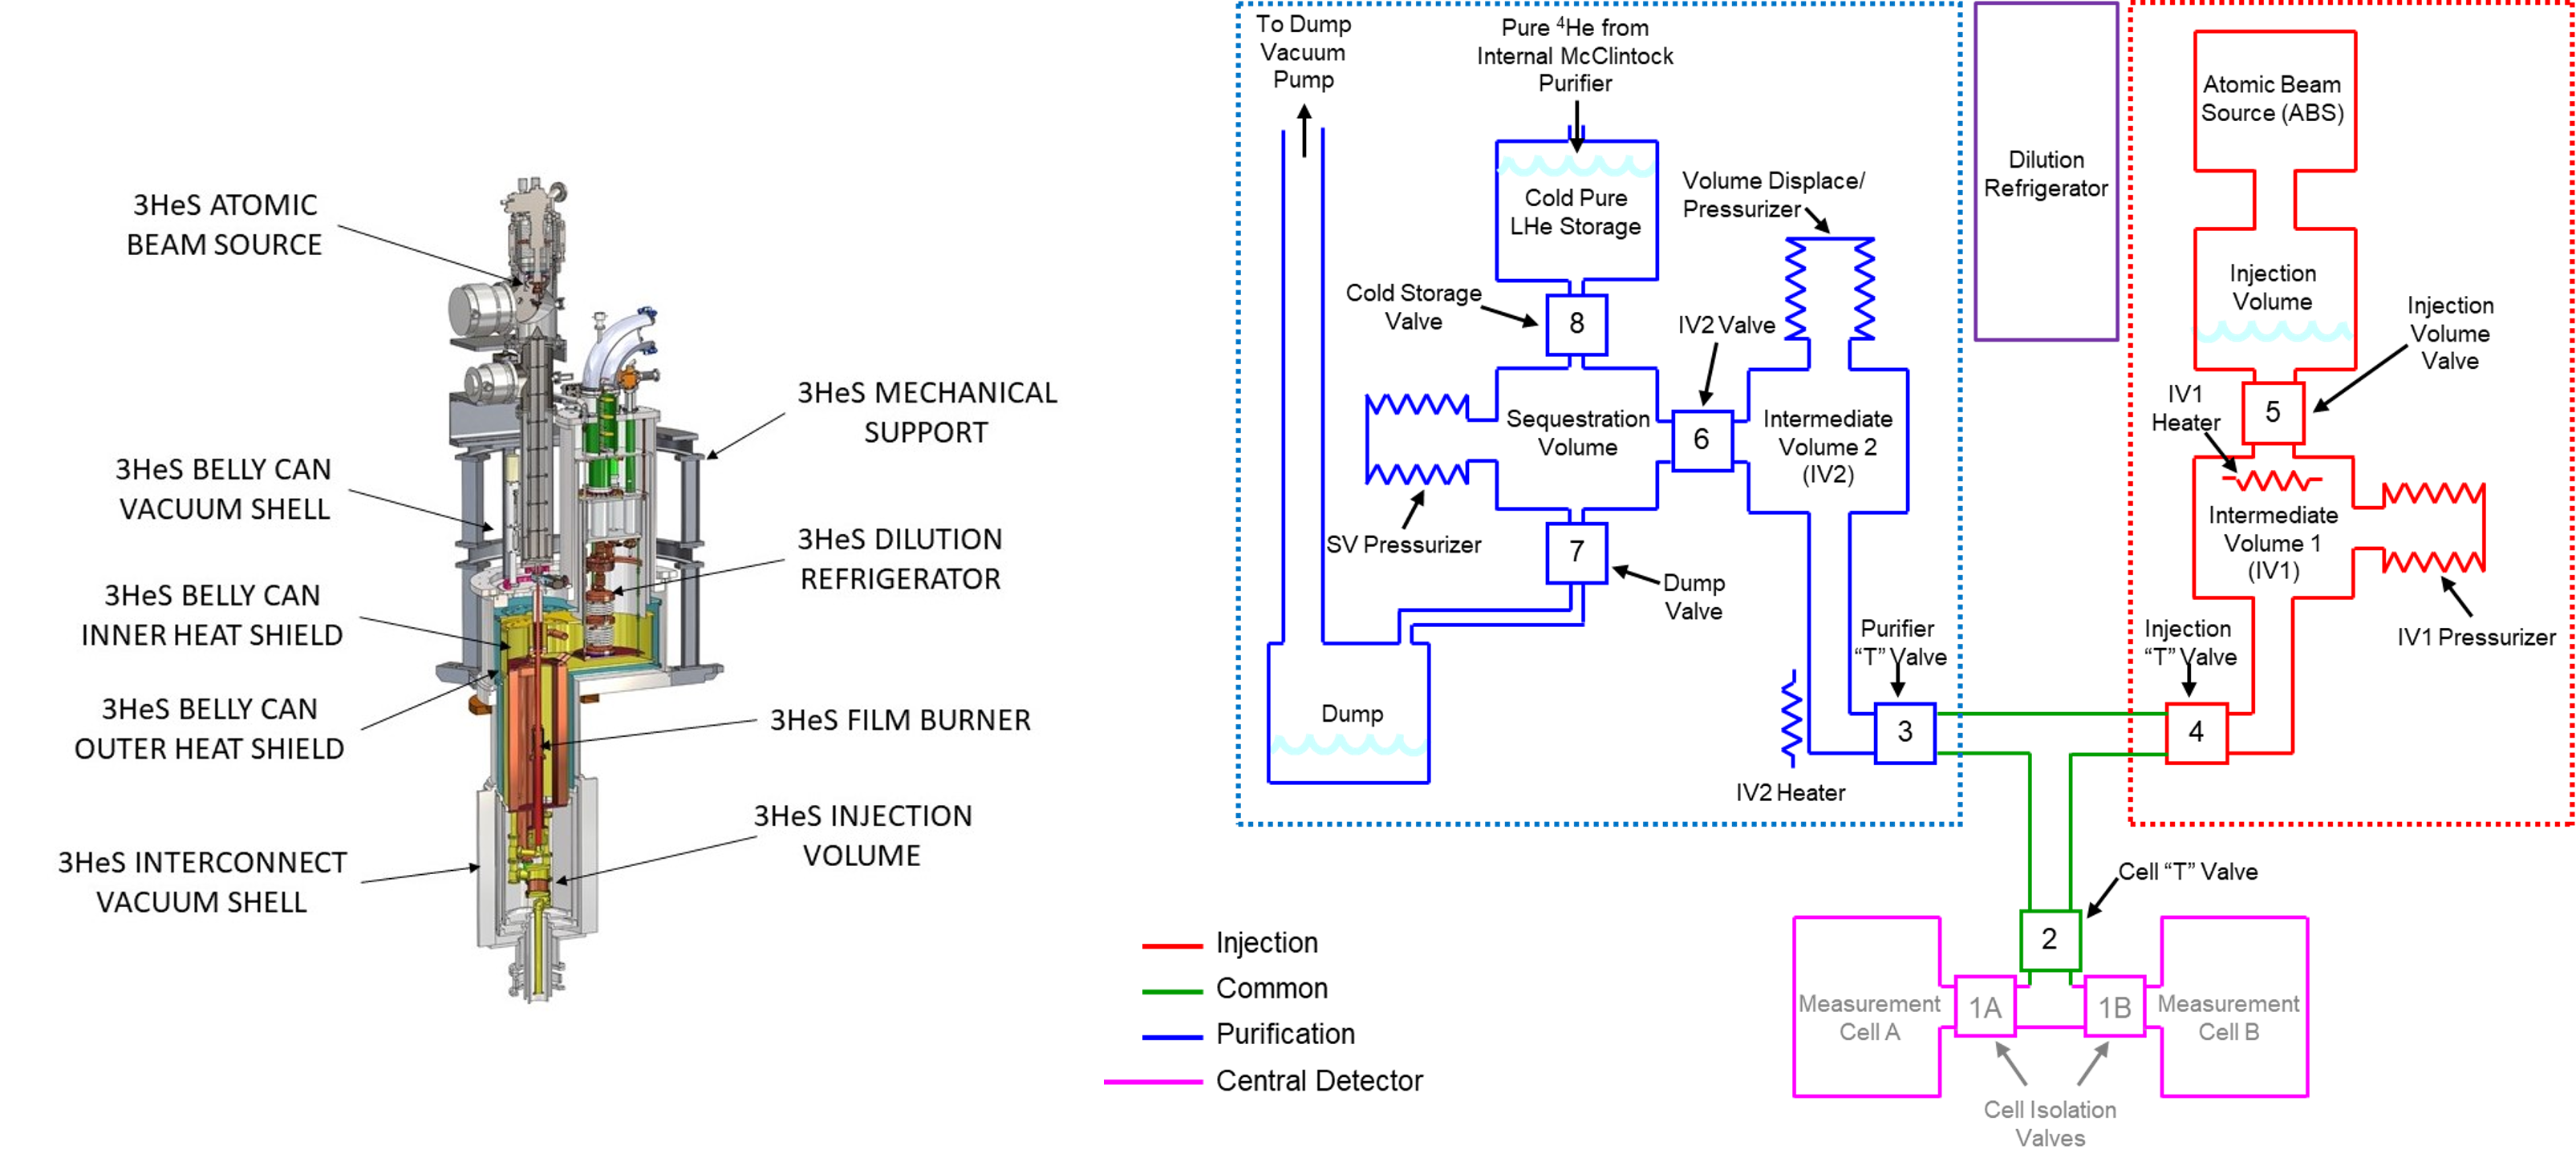
\includegraphics[width=1\textwidth]{figures/chapter2-figs/3He_detail.png}
    \caption[Overall schematic of the polarized $^3$He subsystem.]{Overall schematic of the polarized $^3$He subsystem. Figure on the left is taken from \cite{Ahmed2019} and figure on the right is courtesy of Steve Williamson of the nEDM@SNS collaboration.}
    \label{fig:3He_sys}
\end{figure}
\clearpage}

\subsection{Magnetic Field Module System}

The Magnetic Field Module (MFM), which surrounds the CDS, is responsible for providing all of the magnetic fields relevant for the spin precession measurements as well as the appropriate magnetic shielding. A schematic of this system is shown in \cref{fig:MFM}. 

\afterpage{
\begin{figure}
    \centering
    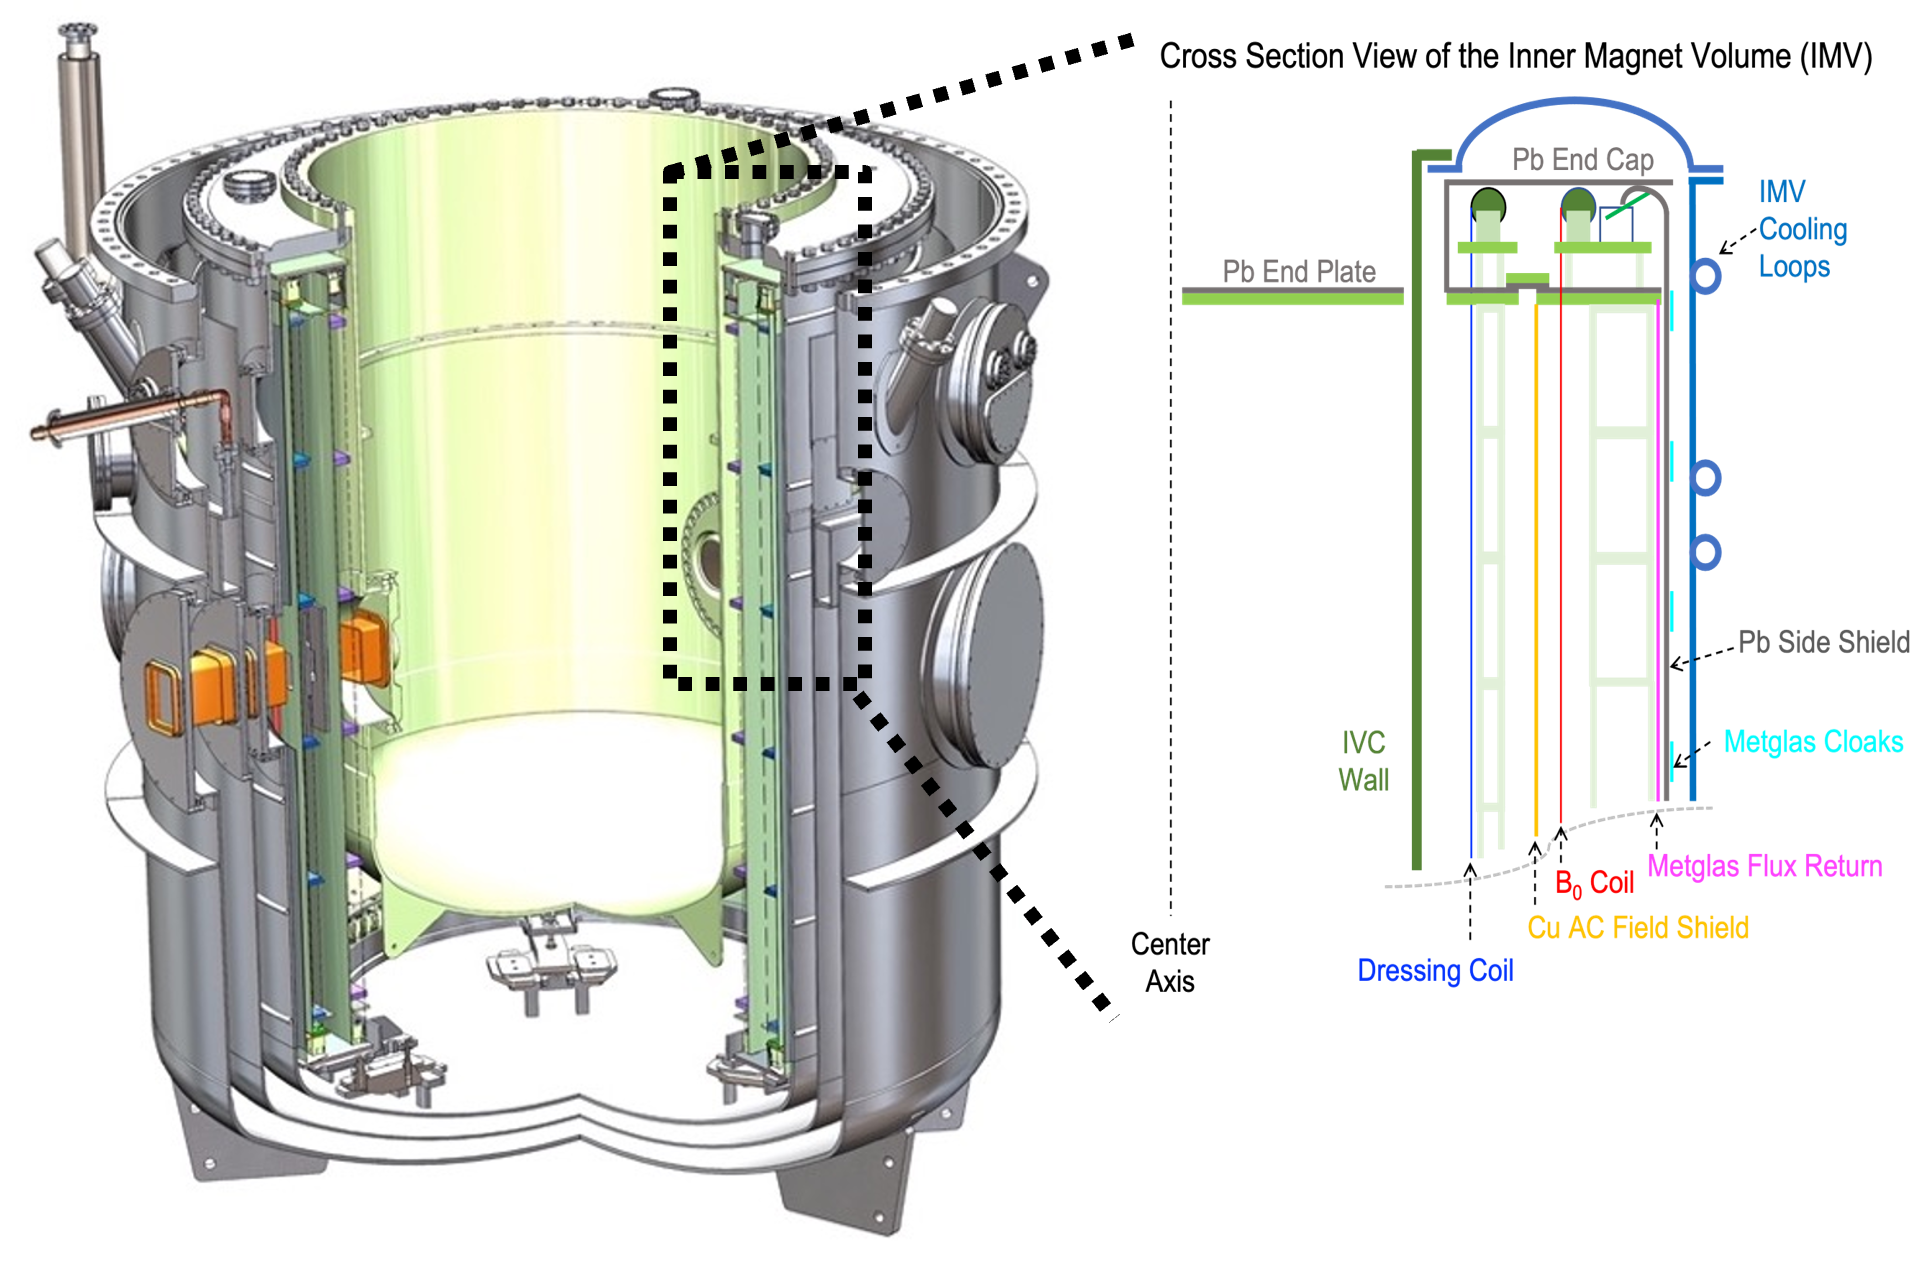
\includegraphics[width=1\textwidth]{figures/chapter2-figs/MFM.png}
    \caption[Overall schematic of the Magnetic Field Module system.]{Overall schematic of the Magnetic Field Module system. Figure taken from \cite{Ahmed2019}.}
    \label{fig:MFM}
\end{figure}
\clearpage}

Going outwards from the center, the vertical concentric cylindrical components of the MFM are: the spin dressing cos$\theta$ coil to provide RF fields, transverse to $B_0$ magnetic field, for the $\pi$/2 rotation and spin dressing, a thin conductor eddy current shield to reduce heating from the spin dressing field, a cos$\theta$ $B_0$ coil to provide the uniform 30 mG field in the horizontal direction, a ferromagnetic shield made of high permeability material, Metglas, to provide a flux return for the $B_0$ field and improving the $B_0$ uniformity, and lastly a superconducting Pb magnetic shield for eliminating time varying drifts in the magnetic fields. Two Pb layers cap the top and bottom ends of the MFM with the return loops of the $B_0$ coil on the outside to mimic the $B_0$ coil if it were of infinite length and further improve the field uniformity. The expected magnetic field gradients based on the design are less than $1\times 10^{-7}$ G cm$^{-1}$. A schematic of the fields produced by the MFM is shown in \cref{fig:MFM_Bfields}. A cylindrical array of fluxgate magnetometers will be located between the MFM and the CDS \cite{Ahmed2019} to allow for coarse tuning of magnetic field gradients.

\afterpage{
\begin{figure}
    \centering
    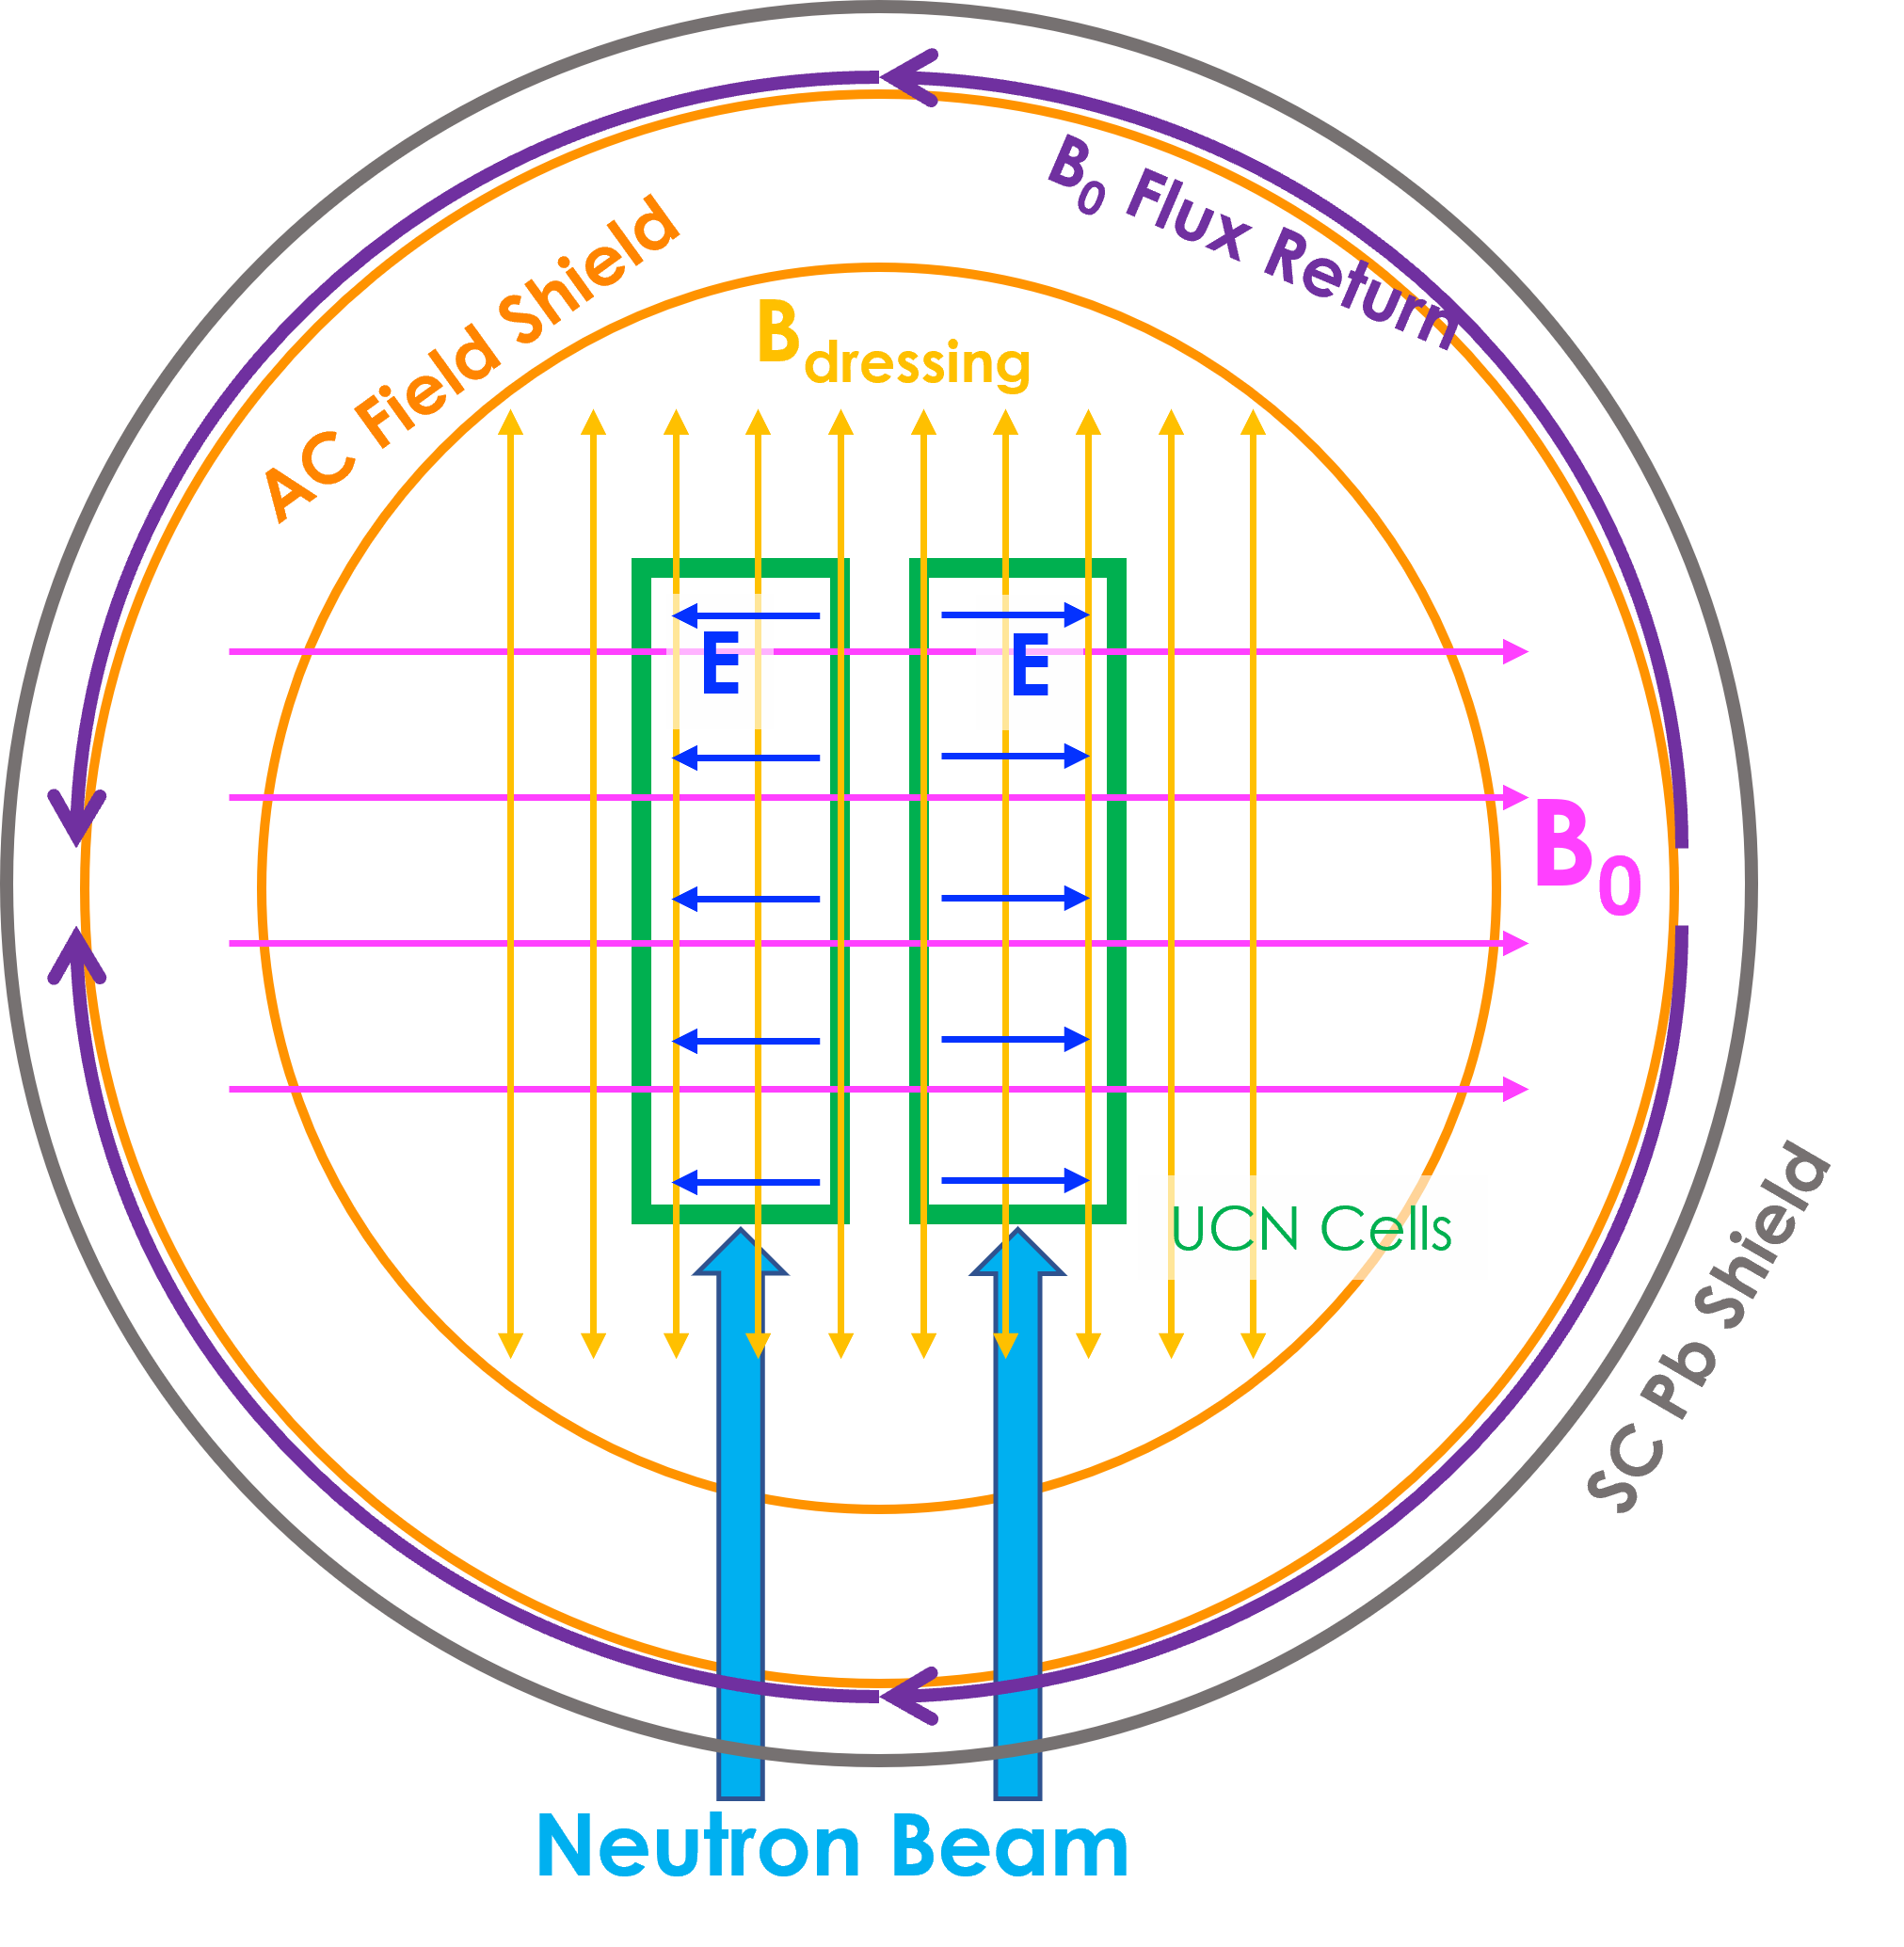
\includegraphics[width=1\textwidth]{figures/chapter2-figs/MFM_Bfields.png}
    \caption{A top down cross-sectional view of the main magnetic field generating components of the Magnetic Field Module. Figure courtesy of Wanchun Wei of the nEDM@SNS collaboration.}
    \label{fig:MFM_Bfields}
\end{figure}
\clearpage}

The next set of the outer layers form the cryostat of the MFM, which consist of the inner magnet volume (IMV) which operates at 4 K, the liquid nitrogen shield (LN$_2$ shield), which operates at 77 K and reduces radiative heat load on the IMV and lastly, the outer vacuum chamber (OVC), which forms the vacuum boundary as well as prevents conductive warming of the low-temperature components.

The entire nEDM@SNS apparatus (CDS, MFM and polarized $^3$He system) will reside inside a large 4 m by 4m wide and 6 m tall multi-layered ferromagnetic Magnetic Shield Enclosure (MSE) made of high permeability material called mu-metal. This MSE is shown in \cref{fig:key_nEDM@SNS}. The purpose of the MSE is to provide a less than $1\times 10^{-5}$ G m$^{-1}$ field gradient and a high shielding factor for external RF fields at its center, where the measurement cells will reside. Outside the MSE will be coil pairs along the orthogonal axes of the MSE to cancel out the earth’s magnetic field.

The major components of the apparatus described exist and are expected to undergo full assembly in the upcoming years, with the first nEDM measurement data expected to begin in 2029. As part of this development effort, neutron polarization and transmission measurements need to be performed to check for the neutron intensity and polarization loss from the MFM. These measurements are the main topic of this dissertation and the associated neutron polarimetry is described in the succeeding chapters.